
%%%%%%%%
\section{Key Concepts and Meta Data Constructs}

This section describes the major concepts employed by SilverKing and the corresponding meta
data constructs that support these concepts.

SilverKing stores all metadata in ZooKeeper. Each metadata construct is identified by a name and version. The version is automatically selected by ZooKeeper using its auto-versioning feature. 

\subsection{Topology}

A topology defines a logical hierarchical relationship between entities such as servers, racks, datacenters, etc. A topology is typically constructed to reflect underlying physical constraints such as network latency, failure correlation, etc.

\begin{figure}[tbh]
\vspace{-0.1in}
\begin{center}
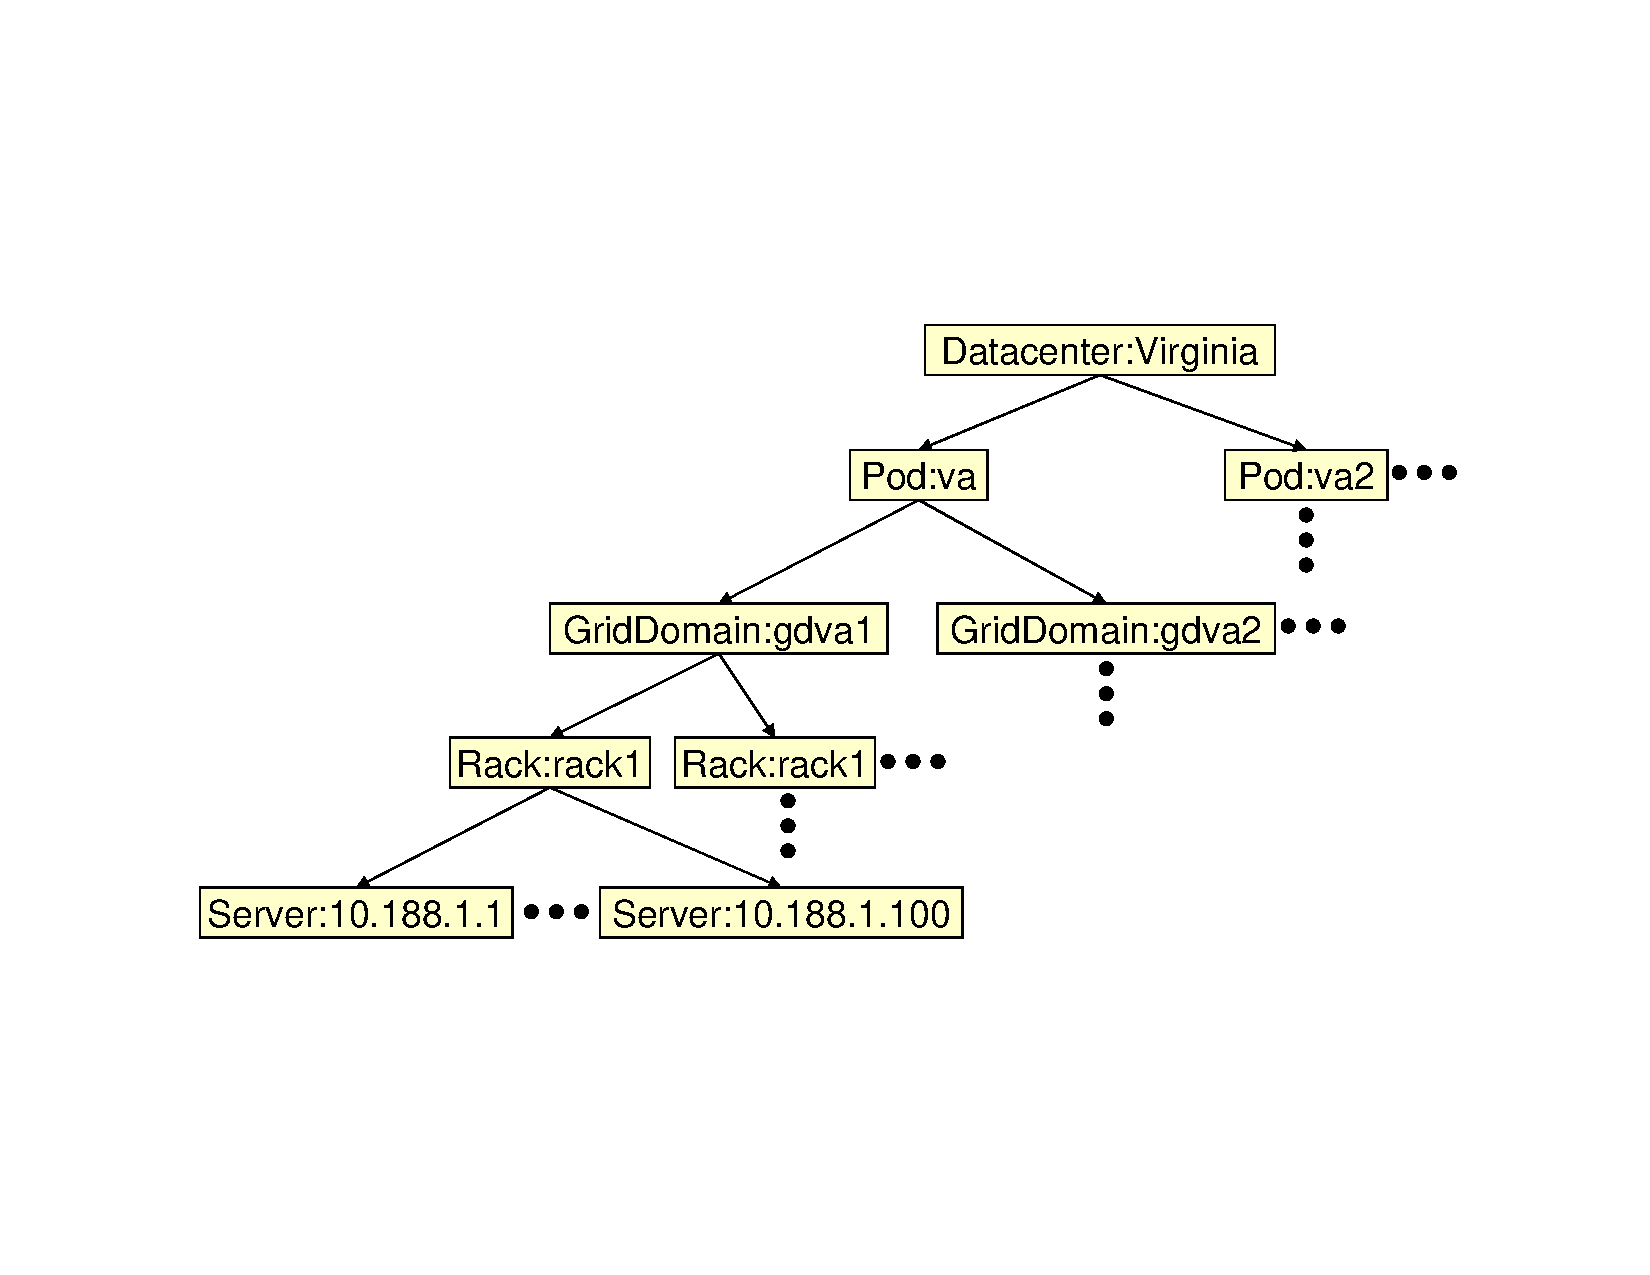
\includegraphics[width=5in, keepaspectration]{Topology.pdf}
\end{center}
\vspace{-0.1in}
\caption{my caption}
\label{fig:Topology}
\vspace{-0.1in}
\end{figure}

\subsection{Exclusions}

Exclusions define a list of servers that should not be included in any ring. Adding a server to the exclusion list precludes data from being stored on the server.

% Rings
\subsection{Rings}

A ring is a logical structure with which key-value pairs are associated. This structure is realized using a range of the integers; each key to be stored in the ring is mapped to one of these integers. 

SilverKing rings are associated with nodes in a topology, and
each non-leaf element in a topology may have a ring associated with it. This node in the topology is referred to as the ring's ``owner''. The topological children of the owner are ``members'' of the ring. Each ring is divided into segments that are ``owned'' by ring members. The segment owners are responsible for storing all data in the segment.

For instance, a rack may have a ring associated with it where the servers in the rack are the ring members.

A ring is specified as a topology, an owner for the ring within the topology, an exclusion list, and two ring-specific constructs: weights and storage policy.

\subsubsection{Weights}

A weight is a positive real number associated with each member of a ring. The total size of the segments owned by each member - and hence the members' share of the overall data - is proportional to their weights. Unless otherwise specified, the default weight is 1.0.

\subsubsection{Storage Policy}

A storage policy defines how data is stored within a ring. Currently, each value is stored in one or more members of the ring using replication. ``Primary'' replicas must store the data item. ``Secondary'' replicas will attempt to store data items, but are not required to.

%DHT
\subsection{DHT}

A DHT is specified as a ring name and a ZooKeeper ensemble specification.



%%%%%%%%
\section{Metadata Mutation}

As base metadata changes, dependendent metadata is updated accordingly. The following dependencies exist:
	ring <== topology, exclusion, 